\chapter{Arquitetura do Projeto}
\label{arq-cap}
Este capítulo descreve o funcionamento de cada componente do GSMART. A
\autoref{esquema-geral} representa um esquema geral dos módulos do projeto, já a
\autoref{diagrama-fluxo} apresenta o mesmo esquema da visão de um diagrama de
fluxo, sendo apontados entidades e processos do sistema.

\begin{figure}[!h]
  \caption{\label{esquema-geral}Arquitetura geral do sistema}
  \begin{center}
    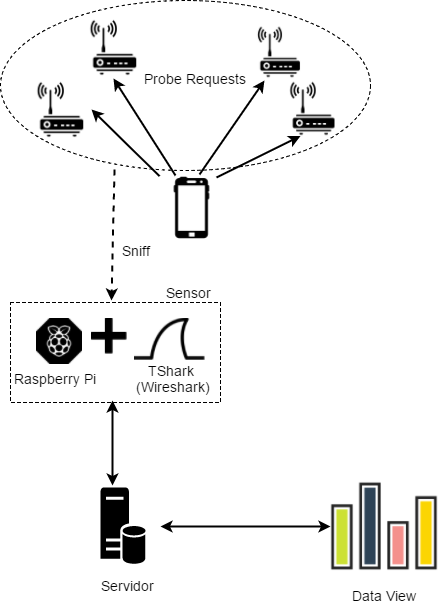
\includegraphics[width=0.50\textwidth]{img/esquema_geral.png}
  \end{center}
  \legend{Fonte: Elaborada pelas autoras.}
\end{figure}

\begin{figure}[!h]
  \caption{\label{diagrama-fluxo}Diagrama de Fluxo}
  \begin{center}
    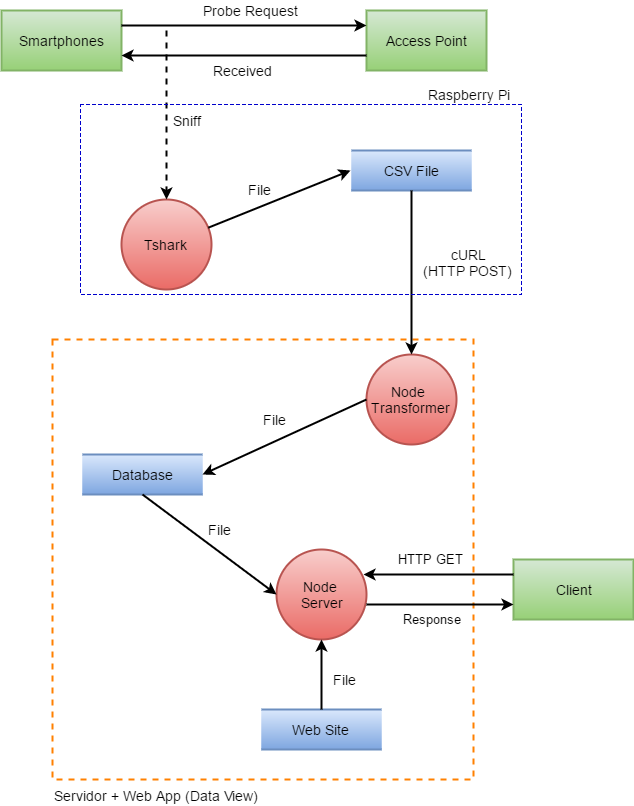
\includegraphics[width=0.70\textwidth]{img/diagrama_fluxo.png}
  \end{center}
  \legend{Fonte: Elaborada pelas autoras.}
\end{figure}


\section{Sensor}
\label{secao-sensor}
O módulo Sensor é um processo que roda num Raspberry Pi Model 3 B equipado de
uma antena Ralink no modo monitor. Este processo é um programa escrito em
Node.js que: habilita o modo monitor da antena, executa comandos Tshark para capturar de pacotes
\emph{probe request}, salva os endereços MAC
capturados num arquivo que, posteriormente, é recuperado do diretório de
arquivos (\emph{Files Directory}) e enviado ao servidor.

\begin{figure}[!h]
  \caption{\label{trecho-sensor}Trecho de código do sensor}
  \begin{center}
    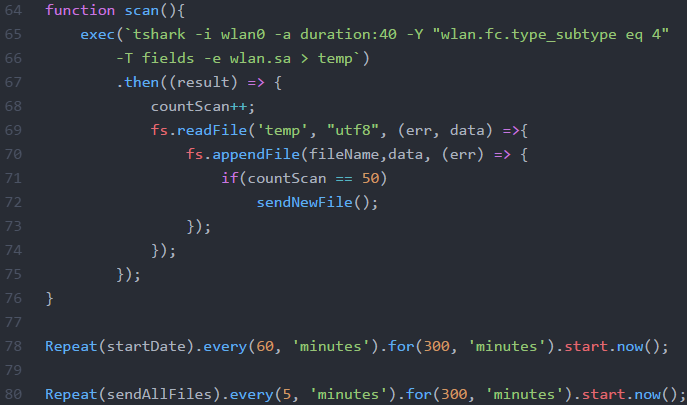
\includegraphics[width=1.0\textwidth]{img/sensor.png}
  \end{center}
  \legend{Fonte: Elaborada pelas autoras.}
\end{figure}

A \autoref{trecho-sensor} contém uma parte do código que executa dentro do
sensor. Ele funciona em 3 fluxos:

\begin{itemize}
    \item \textbf{startDate}: esse fluxo, representado na linha 78
    do código, executa a função "startDate" cada 60 minutos, criando um arquivo com
    o nome "ZONA\_YYYY-MM-DD\_HH:00", especificando zona, dia e hora de detecção. Logo
    após, salva o arquivo e inicia o fluxo a seguir;
    \item \textbf{scan}: este fluxo (linha 78) repete a função "scan" a cada 40 segundos durante 50 minutos que executa o
    comando Tshark (veja \autoref{tshark-section}) que vai armazenando os endereço
    MAC num arquivo temporário. Quando as execuções do Tshark chegam na contagem 50
    o conteúdo do arquivo  é copiado para o arquivo gerado no fluxo anterior, então é enviado ao servidor;
    \item \textbf{sendAllFiles}: este fluxo (linha 80) repete a função "sendAllFiles" a cada 5 minutos enviando todos os arquivos que tiveram falha no seu
    primeiro envio.
    capturado.
\end{itemize}

\section{Node Transformer}
\label{node-transformer}
Após receber o arquivo, o servidor salva-o no diretório e encaminha os endereços MAC capturados para o
módulo de transformação.

O Node Transformer é um módulo dentro do \emph{webserver}
que transforma os endereços MAC em dados formatados.
de dados. Primeiro, são eliminadas os endereços repetidos. Depois, a estrutura de dado (objeto)
que representa um registro do banco é preenchida com a informações. Uma parte importante dessa preparação
é que o fabricante de cada dispositivo é obtido através de uma API\footnote{\url{https://macvendors.com/}} de consulta de endereços MAC. Por fim,
o objeto preenchido é salvo no banco de dados.

\subsection{Formatação do dado}
A formatação do dado foi pensada de acordo com a unidade de tratamento escolhida para a medição tráfego, o dia.
Dentro da aplicação e do banco, o dado possui o formato do JSON da \autoref{formatacao-dado}.

\begin{figure}[!h]
  \caption{\label{formatacao-dado}Formatação do dado}
  \begin{center}
    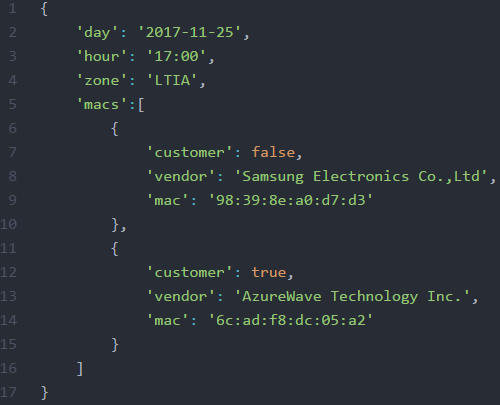
\includegraphics[width=0.8\textwidth]{img/formato-dado.png}
  \end{center}
  \legend{Fonte: Elaborada pelas autoras.}
\end{figure}

Cada objeto como o da \autoref{formatacao-dado}, possui os seguintes campos sobre a medição:
\begin{itemize}
    \item \textbf{day}: dia;
    \item \textbf{hour}: hora;
    \item \textbf{zone}: zona em que foi realizada;
    \item \textbf{macs}: vetor de todos os endereços MAC capturados;
    \item \textbf{customer}: se o endereço captado já foi capturado outro(s) dia(s);
    \item \textbf{vendor}: fabricante do dispositivo;
    \item \textbf{mac}: endereços MAC.
\end{itemize}

O maior ganho com essa formatação é durante as \emph{queries} e processamento dos dados. O dado pode ser recuperado
por zona ou por dia, dependendo da visualização de dados selecionada.

\section{Node Server}
\label{node-server}


\section{Visualização de Dados}
\label{data-view}

\section{Arquiteturas específicas}
-api
-rest
-MVC
%
% \subsection{Node Transformer}
% \label{node-transformer}
% Após converter os dados do pacotes recebidos para um arquivo, o
% Raspberry Pi dá um cURL POST (HTTP POST através do terminal) de tempos em tempos
% para enviar o arquivo daquela sessão ao servidor. No servidor, o módulo
% node transformer particionará o arquivo (segundo alguns campos) em outros
% arquivos .JSON, que serão salvos no banco de dados.
%
% \subsection{Node Server}
%  A partir dos arquivos .JSON citados no item anterior e um Web Site base (HTML,
%  CSS, Javascript), o módulo Node Server responde (Response) à requisição do
%  cliente (HTTP GET) e apresenta-o os dados capturados.
%
% \section{Data View}
% O Data View é a parte do Web App responsável por apresentar os dados capturados
% de maneira clara e legível. Para isso, a biblioteca D3.js \cite{D32017} será
% utilizada para a plotagem de gráficos a partir dos arquivos .JSON.
%
